\documentclass{article}
\usepackage{assignment_preamble}

\title{Lab 1}
\author{Ravi Kini}
\date{October 15, 2023}

\begin{document}

\maketitle

\repository{https://github.com/ravidosa/notes/tree/main/academics/assignments/code/phy112l_lab1}

\problem
A system with a finite set of $N$ energy states $E_0, \ldots E_{N-1}$ at a temperature $T$ has the partition function:
\begin{equation}
    Z = \sum_{n = 0}^{N - 1} e^{-\beta E_n}
\end{equation}
where $\beta = \frac{k_B}{T}$ and $k_B = 1.38 \cdot 10^{-23}~\unit{\joule\per\kelvin}$ is Boltzmann's constant. The probability the system is in state $n$ with energy $E_n$ is then:
\begin{equation}
    p_n = \frac{e^{-\beta E_n}}{Z}
\end{equation}
Summing this probability over all values of $n$:
\begin{equation}
    \begin{split}
        \sum_{n=0}^{N-1} p_n & = \sum_{n=0}^{N-1} \frac{e^{-\beta E_n}}{Z} \\
        & = \frac{\sum_{n=0}^{N-1} e^{-\beta E_n}}{Z} \\
        & = \frac{\sum_{n=0}^{N-1} e^{-\beta E_n}}{\sum_{n=0}^{N-1} e^{-\beta E_n}} = 1
    \end{split}
\end{equation}
This makes sense; the system has to be in exactly one of the states at any given time. Since the events of being in any given state are pairwise disjoint and comprise the entire sample space, the sum of their probabilities equals the probability of their union, which constitutes the whole sample space and is therefore 1.

\clearpage

\problem
In the high-temperature limit, $T \to \infty, \beta \to 0$. In the high-temperature limit, the partition function $Z$ becomes:
\begin{equation}
    \begin{split}
        \lim_{T\to\infty} Z & = \lim_{\beta\to 0} Z = \lim_{\beta\to 0} \sum_{n=0}^{N-1} e^{-\beta E_n} \\
        & = \lim_{\beta\to 0} \sum_{n=0}^{N-1} {\left(e^{- E_n}\right)}^{\beta} \\
        & = \sum_{n=0}^{N-1} {\left(e^{- E_n}\right)}^{0} = \sum_{n=0}^{N-1} 1 = N \\
    \end{split}
\end{equation}
In the high-temperature limit, the probability $p_n$ becomes:
\begin{equation}
    \begin{split}
        \lim_{T\to\infty} p_n & = \lim_{\beta\to 0} p_n = \lim_{\beta\to 0} \frac{ e^{-\beta E_n}}{Z} \\
        & = \frac{\lim_{\beta\to 0} {\left(e^{- E_n}\right)}^{\beta}}{\lim_{\beta\to 0} Z} = \frac{\lim_{\beta\to 0} e^{-\beta E_n}}{N} \\
        & = \frac{{\left(e^{- E_n}\right)}^{0}}{N} = \frac{1}{N} \\
    \end{split}
\end{equation}
At high temperatures, the system has an equal probability of being in any given state.

\clearpage

\problem
Suppose the energy states are shifted by some $\mathcal{E}$. Then:
\begin{equation}
    \begin{split}
        p_n' & = \frac{e^{-\beta (E_n + \mathcal{E})}}{\sum_{i=0}^{N-1} e^{-\beta (E_i + \mathcal{E})}} \\
        & = \frac{e^{-\beta\mathcal{E}}e^{-\beta E_n}}{\sum_{i=0}^{N-1} e^{-\beta\mathcal{E}}e^{-\beta E_i}} = \frac{e^{-\beta\mathcal{E}}e^{-\beta E_n}}{e^{-\beta\mathcal{E}}\sum_{i=0}^{N-1} e^{-\beta E_i}} \\
        & = \frac{e^{-\beta E_n}}{\sum_{i=0}^{N-1} e^{-\beta E_i}} = \frac{e^{-\beta E_n}}{Z} = p_n
    \end{split}
\end{equation}
Evidently, the probabilities are unchanged.

\clearpage

\problem

Shifting the energy states by $\mathcal{E} = -E_0$, in the low-temperature limit, the probability $p_n$ becomes:
\begin{equation}
    \begin{split}
        E_n' & = E_n - E_0 \\
        \lim_{T\to 0} p_n & = \lim_{\beta\to\infty} p_n = \lim_{\beta\to\infty} \frac{ e^{-\beta E_n}}{Z} \\
        & = \lim_{\beta\to\infty} \frac{e^{-\beta E_n}}{\sum_{i=0}^{N-1} e^{-\beta E_i}} \\
        & = \lim_{\beta\to\infty} \frac{e^{-\beta E_n'}}{\sum_{i=0}^{N-1} e^{-\beta E_i'}} \\
        & = \lim_{\beta\to\infty} \frac{e^{-\beta E_n'}}{1 + \sum_{i=1}^{N-1} e^{-\beta E_i'}} \\
        & = \frac{\lim_{\beta\to\infty} e^{-\beta E_n'}}{\lim_{\beta\to\infty} 1 + \sum_{i=1}^{N-1} e^{-\beta E_i'}} = \lim_{\beta\to\infty} e^{-\beta E_n'} \\
        & = \begin{cases}
            1 & n = 0 \\
            0 & n \neq 0
        \end{cases}
    \end{split}
\end{equation}
At low temperatures, the system is in the state with the lowest energy.

\clearpage

\problem
Since the zero of potential energy should not affect the behaviour of the system, we can approximate the low-temperature limit as $\frac{k_B T}{E_n - E_0} \ll 1$.

\clearpage

\problem
The average energy of the system is:
\begin{equation}
    \langle E \rangle = \sum_{n=0}^{N-1}p_n E_n = \frac{1}{Z}\sum_{n=0}^{N-1}E_n e^{-\beta E_n}
\end{equation}
This can also be expressed as:
\begin{equation}
    \begin{split}
        -\deriv[]{}{\beta} \ln{Z} & = -\frac{1}{Z}\deriv[]{Z}{\beta} \\
        & = -\frac{1}{Z}\deriv[]{}{\beta}\sum_{n=0}^{N-1} e^{-\beta E_n} \\
        & = -\frac{1}{Z}\sum_{n=0}^{N-1} \deriv[]{}{\beta} e^{-\beta E_n} \\
        & = -\frac{1}{Z}\sum_{n=0}^{N-1} -E_n e^{-\beta E_n} \\
        & = \frac{1}{Z}\sum_{n=0}^{N-1} E_n e^{-\beta E_n} = \langle E \rangle
    \end{split}
\end{equation}

\clearpage

\problem
The program outputs:
\begin{center}
    \begin{tabular}{|c|c|}
        \hline
        $T$ & $\langle E \rangle$ \\
        \hline
        0.3 & 2.629031591439724 \\
        \hline
        2.0 & 3.289391079764234 \\
        \hline
        15.0 & 3.502166085220926 \\
        \hline
    \end{tabular}
\end{center}

\clearpage

\problem
Figure \ref{fig:fig1} is a plot of $\langle E \rangle$ vs. $T$  for $N = 3$ and $E_0 = 0.7, E_1 = 1.3, E_2 = 5.0$. As $T \to \infty$, $\langle E \rangle \to \frac{\sum_{n=0}^{N-1}E_n}{N} = \frac{7}{3} \approx 2.33$. This makes sense in terms of the result for Exercise 2, as $p_n = \frac{1}{N}$ for all $n$ at high temperatures, so $\langle E \rangle = \sum_{n=0}^{N-1}p_n E_n = \frac{\sum_{n=0}^{N-1}E_n}{N}$. As $T \to 0$, $\langle E \rangle \to E_0$. This makes sense in terms of the result for Exercise 4, as $p_0 = 1$ and $p_n = 0$ for all $n \neq 0$ at low temperatures, so $\langle E \rangle = \sum_{n=0}^{N-1}p_n E_n = E_0$. When $M \to \infty$, we model a system that is being heated or cooled.

\begin{figure}[!htb]
    \begin{centering}
    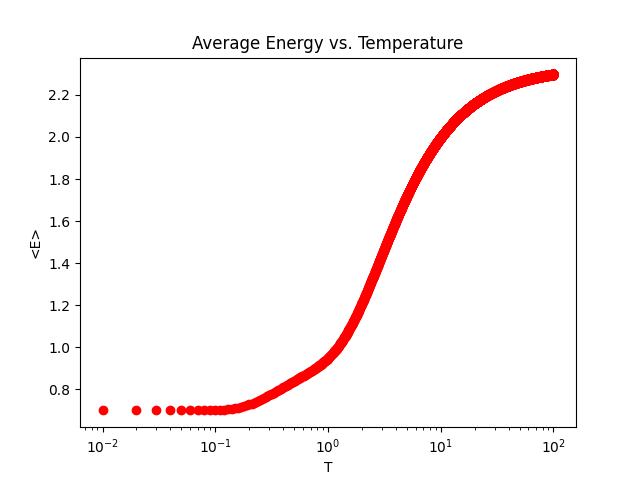
\includegraphics[width=0.75\textwidth]{../code/phy112l_lab1/1-8.png}
    \caption{Plot of average energy vs. temperature  ($E_0 = 0.7, E_1 = 1.3, E_2 = 5.0$).}
    \label{fig:fig1}
    \end{centering}
\end{figure}

\skipproblem

\clearpage

\problem
Figure \ref{fig:fig2} is a plot of $C$ vs. $T$ for $N = 2$ and $E_0 = -3.4, E_1 = -3.0$ (peak at $T = 0.16$). Figure \ref{fig:fig3} is a plot of $C$ vs. $T$  for $N = 2$ and $E_0 = -3.4, E_1 = 5.0$ (peak at $T = 3.5$).
\begin{equation}
    \begin{split}
        \frac{3.5 - 0.16}{8.4 - 0.4} = 0.4175
    \end{split}
\end{equation}
For a two level system, the peak in $C(T)$ occurs at approximately $T = 0.4175(E_1 - E_0)$.

\begin{figure}[!htb]
    \centering
    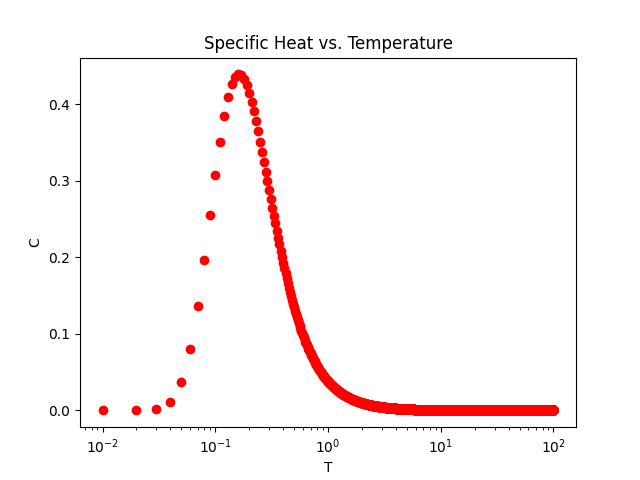
\includegraphics[width=0.75\textwidth]{../code/phy112l_lab1/1-10a.png}
    \caption{Plot of specific heat vs. temperature ($E_0 = -3.4, E_1 = -3.0$).}
    \label{fig:fig2}
\end{figure}
\begin{figure}[!htb]
    \centering
    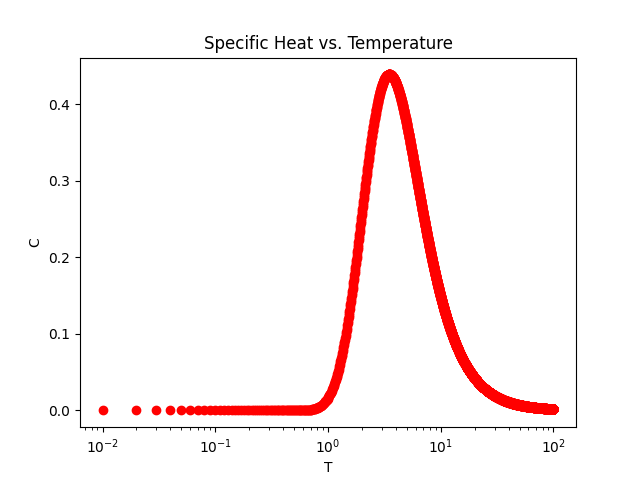
\includegraphics[width=0.75\textwidth]{../code/phy112l_lab1/1-10b.png}
    \caption{Plot of specific heat vs. temperature($E_0 = -3.4, E_1 = 5.0$).}
    \label{fig:fig3}
\end{figure}

\clearpage

\problem
Let $\langle E^2 \rangle = \frac{\sum_{n=0}^{N-1} E_n^2e^{-\beta E_n}}{Z}$.
\begin{equation}
    \begin{split}
        C = \deriv[]{\langle E \rangle}{T} & = \deriv[]{}{T} \frac{\sum_{n=0}^{N-1} E_n e^{-\beta E_n}}{Z} \\
        & = \deriv[]{}{T} \frac{\sum_{n=0}^{N-1} E_n e^{-\beta E_n}}{\sum_{n=0}^{N-1} e^{-\beta E_n}} \\
        & = \frac{\deriv[]{}{T}\sum_{n=0}^{N-1} E_n e^{-\beta E_n} \cdot \sum_{n=0}^{N-1} e^{-\beta E_n} - \sum_{n=0}^{N-1} E_n e^{-\beta E_n} \cdot \deriv[]{}{T}\sum_{n=0}^{N-1} e^{-\beta E_n}}{{\left(\sum_{n=0}^{N-1} e^{-\beta E_n}\right)}^2} \\
        & = \frac{\sum_{n=0}^{N-1} E_n^2\beta^2e^{-\beta E_n} \cdot \sum_{n=0}^{N-1} e^{-\beta E_n} - \sum_{n=0}^{N-1} E_n e^{-\beta E_n} \cdot \sum_{n=0}^{N-1} E_n\beta^2e^{-\beta E_n}}{{\left(\sum_{n=0}^{N-1} e^{-\beta E_n}\right)}^2} \\
        & = \frac{\beta^2\sum_{n=0}^{N-1} E_n^2e^{-\beta E_n} \cdot \sum_{n=0}^{N-1} e^{-\beta E_n} - \beta^2{\left(\sum_{n=0}^{N-1} E_n e^{-\beta E_n}\right)}^2}{{(\sum_{n=0}^{N-1} e^{-\beta E_n})}^2} \\
        & = \beta^2\frac{\sum_{n=0}^{N-1} E_n^2e^{-\beta E_n} \cdot Z - {\left(\sum_{n=0}^{N-1} E_n e^{-\beta E_n}\right)}^2}{Z^2} \\
        & = \beta^2\left(\frac{\sum_{n=0}^{N-1} E_n^2e^{-\beta E_n}}{Z} - {\left(\frac{\sum_{n=0}^{N-1} E_n e^{-\beta E_n}}{Z}\right)}^2\right) \\
        & = \beta^2\left(\langle E^2 \rangle - \langle E \rangle^2\right)
    \end{split}
\end{equation}

\clearpage

\problem
Figure \ref{fig:fig4} is a plot of $C$ vs. $T$  for $N = 2$ and $E_0 = -3.4, E_1 = -3.0$. Figure \ref{fig:fig5} is a plot of $C$ vs. $T$  for $N = 2$ and $E_0 = -3.4, E_1 = 5.0$. The FDT approach is advantageous at low values of $T$, where $T$ changes rapidly and $dT$ may not be small enough for a good approximation of $C$. Further, if the measurements of $\langle E \rangle$ have error bars, the derivative method will have a larger error in its computed value of $C$; however, the FDT approach avoids this issue as derivatives are not used. Suppose, in a Monte Carlo simulation that aims to measure the specific heat, we take $M$ random samples ($E_i \pm \sigma$) at the target temperature $T$ and $M$ random samples ($E_i' \pm \sigma$) at the temperature $T + dT$. The uncertainties are then as follows:
\begin{equation}
    \begin{split}
        \sigma_{\langle E \rangle} & = \frac{\sigma}{\sqrt{M}}, \sigma_{\langle E' \rangle} = \frac{\sigma}{\sqrt{M}},
        \sigma_{\langle E^2 \rangle}  = \frac{2\sigma}{M}\sqrt{\sum_i E_i^2} \\
        \sigma_{deriv} & = \frac{\frac{\sigma}{\sqrt{M}} + \frac{\sigma}{\sqrt{M}}}{dT} = \frac{2\sigma}{dT\sqrt{M}} \\
        \sigma_{FDT} & = \beta^2\left(\frac{2\sigma}{M}\sqrt{\sum_i E_i^2} + \frac{\sigma^2}{M}\right) = \frac{\beta^2(2E_{RMS} + \sigma)\sigma}{\sqrt{M}}
    \end{split}
\end{equation}
Since good approximations for the specific heat require low values of $dT$, the uncertainty found using the derivative method will greatly exceed that found using the FDT method, as $\frac{2}{dT} \gg \frac{\beta^2\left(2E_{RMS} + \sigma\right)}{T^2}$ for low values of $dT$.

\begin{figure}[!htb]
    \centering
    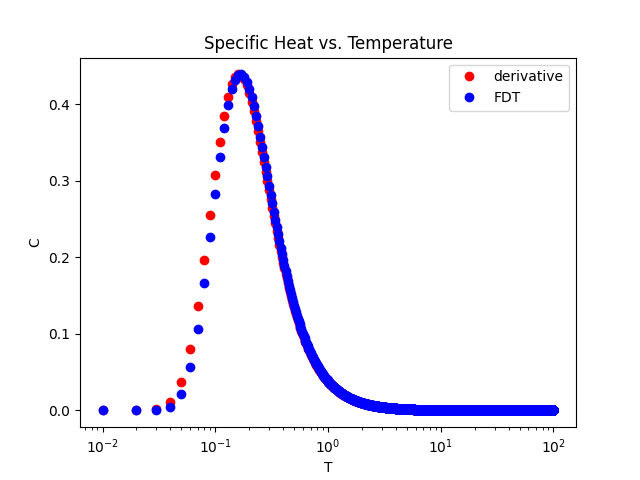
\includegraphics[width=0.75\textwidth]{../code/phy112l_lab1/1-12a.png}
    \caption{Plot of specific heat vs. temperature($E_0 = -3.4, E_1 = -3.0$).}
    \label{fig:fig4}
\end{figure}
\begin{figure}[!htb]
    \centering
    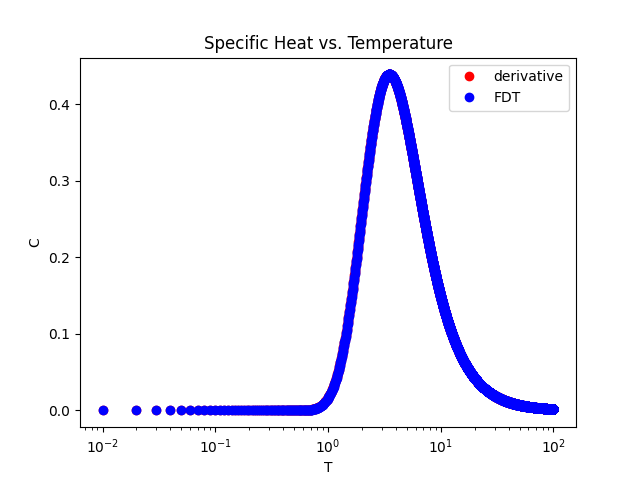
\includegraphics[width=0.75\textwidth]{../code/phy112l_lab1/1-12b.png}
    \caption{Plot of specific heat vs. temperature($E_0 = -3.4, E_1 = 5.0$).}
    \label{fig:fig5}
\end{figure}

\end{document}